\documentclass{article}

\usepackage{amsmath, amssymb}
\usepackage{natbib}
\usepackage{subcaption}
\usepackage{graphicx}
\usepackage{color}

\title{Avoiding Flight Delays with Supervised Ranking}
\author{Dan Garant \and John Lalor \and Adam Nelson}
\date{}

\begin{document}
\maketitle

\begin{abstract}

With the amount of data available on flights in the United States, one interesting task is to use this data in order to make predictions about flight performance. However, being able to find the correct features to use from the variety of available features is important when trying to build a model of flight delays. In this project, we look at predicting flight delays from the point of view of the passengers on the flight. We look at the task of predicting flight delays from two points of view: a customer looking for a flight that departs in one month, and a customer looking for a flight that departs tomorrow. The two tasks offer different features in terms of available weather data. We evaluate a number of models for each task, and present results in the form of rankings, where the flight with the lowest chance of having a delay is presented as the top result.

In this work, we examine the task of selecting flights to minimize the risk of encountering a flight delay.
Using features derived from weather, airport, and air carrier characteristics, we employ various supervised learning techniques to rank flights by their probability of experiencing a delay.
\textcolor{red}{...}

\end{abstract}

\section{Introduction}

Being able to determine whether a flight will take off and arrive on time is a question that is well-suited for analysis with machine learning. Air transportation is something that many people deal with regularly, and a huge amount of data is recorded by the U.S. Government for all of the flights that operate in the U.S. Combine that with the data available about weather patterns and weather history and you have a lot of information about the conditions surrounding air travel. For this project, we will explore this data, and attempt to answer the following question: Can we use machine learning to avoid flight delays when traveling by plane? In this report, we will give an overview of the dataset, and briefly describe some of the work done before using it as a resource, we will look at the data from a high level and look at trends and patterns that arise, and we will apply a number of supervised learning methods to the data to attempt to rank flights based on their likelihood of having a delay. The objective is to use the models to identify the flights that are least likely to be delayed. Our analysis will look at flight delay patterns according to two distinct problems: predicting a flight delay for flights leaving tomorrow, and predicting flight delays for flights leaving in one month (e.g. in thirty days).

\section{Data Sources}
\subsection{Bureau of Transportation Dataset}

The original idea for the project came from the 2009 American Statistical Association Joint Statistical Meetings Data Expo [cite]. The challenge was to create a graphical summary of the data, which consisted of flight statistics from October 1987 to April 2008. The submissions for this explored a variety of aspects of the data. (Need to elaborate here).

The data for the expo came from the United States Department of Transportation (DOT). The DOT Bureau of Transportation Statistics (BTS) track flight statistics for domestic flights. For the purposes of our project, we focused on flight statistics from the year 2014, as these flights were more recent than the original expo dataset and still provide a large set of data from which we could obtain conclusions. We obtained the data directly from the BTS website.  

The BTS data includes a large number of data fields. Below we enumerate the fields that we included in our analysis, along with a description of each:

\begin{itemize}
\item Origin Airport and Departure Airport IDs: Unique IDs used to identify the origin and departure airports for each flight in the dataset. 
\item Departure Date: Date of flight. 
\item Month, Day of Month, and Day of Week: Additional date fields at varying levels of detail. These were included in an attempt to determine if there were specific days of the week or other specific periods that could be tied to flight delays. 
\item Carrier ID: Unique ID for the airline of the flight.
\item Scheduled Departure and Arrival Time: Scheduled arrival and departure times for each flight, as provided by the Computer Reservation System (CRS)
\item Distance: Distance of the flight
\end{itemize}

\subsection{Related Work}

As part of the 2009 task, there were a number of submissions that used the dataset in interesting ways. We will briefly discuss the top four submissions for that task here. \cite{wicklin2009congestion} Used SAS Software to provide a number of visualizations of the data, including departure delay heatmaps by month for each of the years included in the data and historical comparisons of flight delays, showing that the number of delays varied widely between years. \cite{hofmann2011delayed} found that Newark airport was the worst offender when it came to flight delays, which one author can back up empirically. \cite{wickham2011tale} looked at two specific airports, Oakland and San Francisco, and compared number of flights between the two airports, looking at trends in flight numbers in the two airports. \cite{dey2009minimizing} modeled the data as a graph in order to predict delays for any origin-destination pair.

\subsection{Supplemental Data}

In addition to the data provided by the BTS, we wanted to augment the feature set for flights by looking at weather patterns for each of the airports to determine the effect that weather might have on flight delays. For our two tasks, this involved obtaining two new sets of features: detailed weather information for the one-day task, and high level weather normals for the one-month task. The intuition here was that if you are looking to predict flight delays for tomorrow's flights, a lot of detailed weather information will be available for tomorrow that is most likely very accurate. One month in advance, however, the weather information is less likely to be accurate, so we instead looked at ten-year normals for the flight dates, in order to get an idea of weather one month in advance.


\section{Exploratory Analysis}

To inform our selection and tuning of supervised learning algorithms for this task, we performed a number of exploratory analyses characterizing the nature of dependence between specific features and the response (departure delay in minutes). First, we investigated characteristics of organizations involved in fulfilling the flight. \textcolor{red}{...}

To gain a high-level understanding of the relationship between the weather features and delays, we fit a generalized additive model \citep{hastie1990generalized} of delay duration (in minutes) to a linear combination of cubic spline transformations of various weather features. Naturally, there are associations between each of the weather characteristics. For instance, humidity will necessarily be high when it is raining. To isolate the \emph{independent} effects of each of the features on the departure delay, we predicted the conditional expectation of delay $D$ with respect to an individual feature $F_i$, holding other features at their mean value:
\begin{align}
    \label{eq:conditional-exp}
    E[D|F_1=\bar{F_1}, F_2=\bar{F_2}, \ldots, F_i = f_i, \ldots, F_n = \bar{F_n}].
\end{align}
Then, sweeping across various settings for $f_i$ and various feature $F_i$ yields a sensible explanatory model of delay with respect to weather characteristics. When stratifying by airport and evaluating (\ref{eq:conditional-exp}) with respect to wind bearing, we find a strong non-linear relationship. This dependence is likely the result of differing runway orientation at various airports. When wind is blowing \emph{across} a runway, take-off and landing is more challenging, and some pilots may opt to defer until winds are more favorable. Each airport may have a different runway orientation, so the model must be capable of capturing interactions between a discrete characteristic (airport) and a real-valued characteristic (wind direction).

\begin{figure}
\centering
\begin{subfigure}{0.45\textwidth}
    \centering
    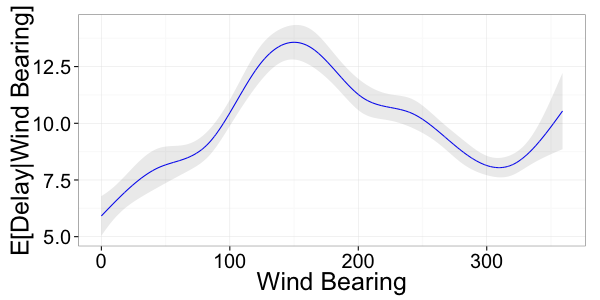
\includegraphics[width=\linewidth]{figures/windBearing-ATL.png}
    \caption{Hartsfield-Jackson Atlanta}
\end{subfigure}
\begin{subfigure}{0.45\textwidth}
    \centering
    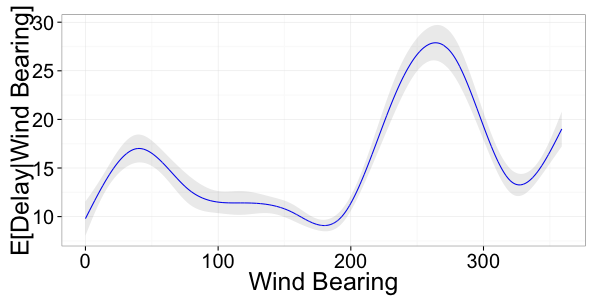
\includegraphics[width=\linewidth]{figures/windBearing-DFW.png}
    \caption{Dallas/Fort Worth}
\end{subfigure}
\begin{subfigure}{0.45\textwidth}
    \centering
    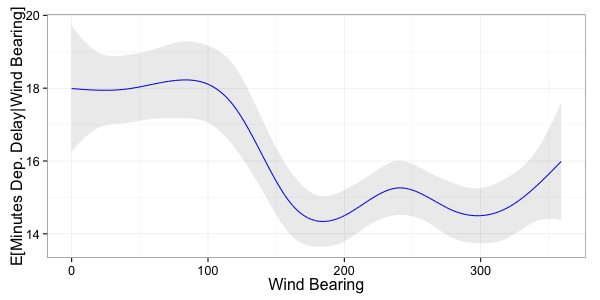
\includegraphics[width=\linewidth]{figures/windBearing-ORD.png}
    \caption{Chicago O'Hare}
\end{subfigure}
\caption{Relationship between wind bearing and expected delays (in minutes) at various airports. One standard error in the conditional expectation is shown in gray.} 
\label{fig:wind-bearing-feature}
\end{figure}

\section{Evaluation Methodology}

\textcolor{red}{
    \begin{itemize}
        \item Features available in each of the two task ``types''
        \item Discussion of evaluation measures: classification accuracy, log-likelihood, ranking accuracy
        \item Learning algorithms under consideration
        \item hyper-parameter optimization
    \end{itemize}
}

\section{Results}

\begin{figure}
    \centering
    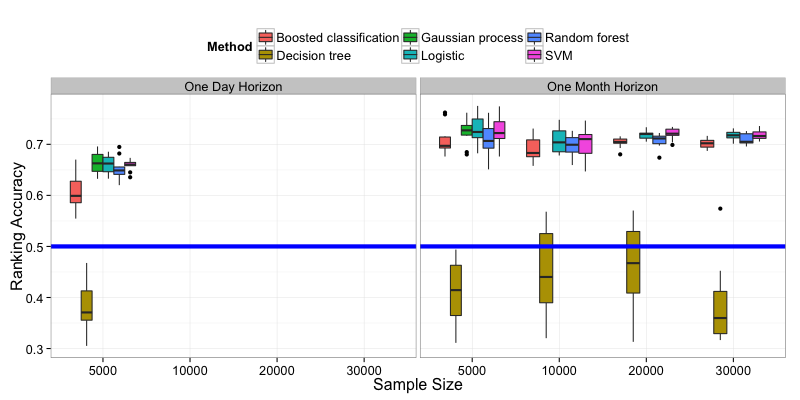
\includegraphics[width=\textwidth]{figures/performance-by-sample-size.png}
    \caption{Ranking accuracy of supervised techniques as sample size is varied}
\end{figure}



\bibliographystyle{plain}
\bibliography{bibliography,bib.bib} 


\end{document}

